\subsection{積圏と一点離散圏}
  一般的に圏は対象の集合や射集合を具体的な元を指定することで定義して、それが公理を満たすか確認していたが、すでに集合や写像は圏論的な操作で扱うことができる。そのため、これから$\cat{Cat}$における積対象となる積圏と、終対象となる一点離散圏、その周辺の関手を集合の圏を用いて定義していく。
	\begin{define}[積圏]
		ある圏$\cat{A,B}$に対する\textbf{積圏}$\cat{A\times B}$を以下の要素で定義する。
		\begin{quote}
			\begin{mydescription}
				\item[対象] \[\obj{A\times B}=\obj{A}\times\obj{B}\]
				すなわち、圏$\cat{A}$と圏$\cat{B}$の任意の対象$A,B$の対$\tuple{A,B}$が$\cat{A\times B}$の対象であり、紛らわしくないように\[\tuple{A,B}=\pcobj{A,B}\]と表記する。

				また$\obj{A}\times\obj{B}$は直積集合であり、集合の圏の積対象であるが、圏$\cat{A\times B}$の対象$\pcobj{A,B}$そのものは積の普遍性を持たないことに注意してほしい。今回積とみなすのは対象ではなく圏の方である。
				\item[射]任意の対象$\pcobj{A,B},\pcobj{A',B'}$に対してその射集合をそれぞれ\[\arset{(A\times B)}{\pcobj{A,B}}{\pcobj{A',B'}}=\arset{A}{A}{A'}\times\arset{B}{B}{B'}\]と定義する。

				すなわち、圏$\cat{A}$の射$\mor{f}{A}{A'}$と圏$\cat{B}$の射$\mor{g}{B}{B'}$の元の対\[\mor{\tuple{f,g}}{[A,B]}{[A',B']}\]が$\cat{A\times B}$の射であり、対象と同様に\[\tuple{f,g}=\pcobj{f,g}\]と表記する。射の対と同じ表記であるが、対象の表記と同様に積の普遍性は持たないため射の対ではない。
				同様に$\arset{A}{A}{A'}\times\arset{B}{B}{B'}$も直積集合であり、集合の圏の積対象である。
				\begin{center}
					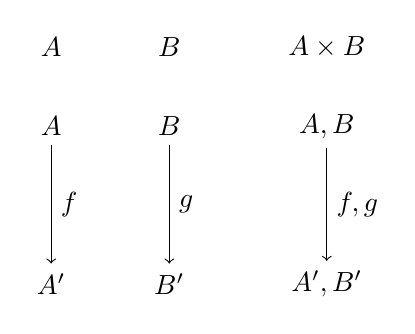
\begin{tikzpicture}[auto]
						\node (a) at (0, 0) {$A$};
						\node (a') at (0, -2) {$A'$};
						\node (b) at (1.5, 0) {$B$};
						\node (b') at (1.5, -2) {$B'$};
						\node (ab) at (3.5, 0) {$\pcobj{A,B}$};
						\node (ab') at (3.5, -2) {$\pcobj{A',B'}$};
						\draw[->] (a) to node{$f$}(a');
						\draw[->] (b) to node{$g$}(b');
						\draw[->] (ab) to node{$\pcobj{f,g}$}(ab');
						\node (cata) at (0, 1) {$\cat{A}$};
						\node (catb) at (1.5, 1) {$\cat{B}$};
						\node (catb) at (3.5, 1) {$\cat{A\times B}$};
					\end{tikzpicture}
				\end{center}
				\item[射の合成] 射$\mor{\pcobj{f,g}}{\pcobj{A,B}}{\pcobj{A',B'}}$と$\mor{\pcobj{f',g'}}{\pcobj{A',B'}}{\pcobj{A'',B''}}$の合成射\[\mor{\pcobj{f',g'}\circ\pcobj{f,g}}{\pcobj{A,B}}{\pcobj{A',B'}}\]を\[\pcobj{f',g'}\circ\pcobj{f,g}=\pcobj{f'\circ f,g'\circ g}\]と定義する。
				\begin{center}
					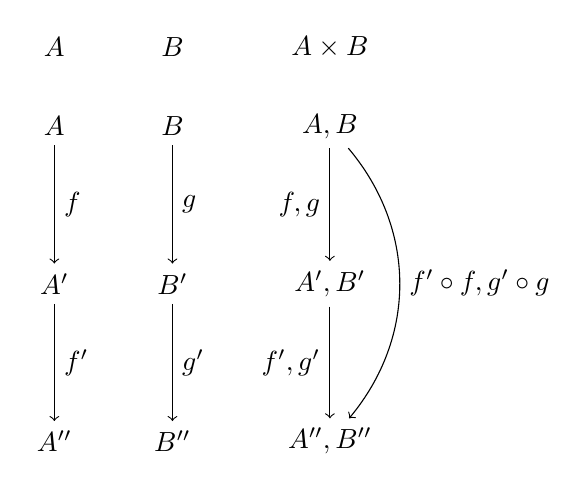
\begin{tikzpicture}[auto]
						\node (a) at (0, 0) {$A$};
						\node (a') at (0, -2) {$A'$};
						\node (a'') at (0, -4) {$A''$};
						\node (b) at (1.5, 0) {$B$};
						\node (b') at (1.5, -2) {$B'$};
						\node (b'') at (1.5, -4) {$B''$};
						\node (ab) at (3.5, 0) {$\pcobj{A,B}$};
						\node (ab') at (3.5, -2) {$\pcobj{A',B'}$};
						\node (ab'') at (3.5, -4) {$\pcobj{A'',B''}$};
						\draw[->] (a) to node{$f$}(a');
						\draw[->] (a') to node{$f'$}(a'');
						\draw[->] (b) to node{$g$}(b');
						\draw[->] (b') to node{$g'$}(b'');
						\draw[->] (ab) to node[swap]{$\pcobj{f,g}$}(ab');
						\draw[->] (ab') to node[swap]{$\pcobj{f',g'}$}(ab'');
						\draw[->,bend left =40] (ab) to node{$\pcobj{f'\circ f,g'\circ g}$}(ab'');
						\node (cata) at (0, 1) {$\cat{A}$};
						\node (catb) at (1.5, 1) {$\cat{B}$};
						\node (catb) at (3.5, 1) {$\cat{A\times B}$};
					\end{tikzpicture}
				\end{center}
				\item[恒等射の存在] 対象$[A,B]$の恒等射$id_{\pcobj{A,B}}$を\[id_{\pcobj{A,B}}=\pcobj{id_A,id_B}\]と定義する。
				\item[結合律]$(\pcobj{f'',g''}\circ\pcobj{f',g'})\circ\pcobj{f,g}=\pcobj{f'',g''}\circ(\pcobj{f',g'}\circ\pcobj{f,g})$を示せばよい。積圏の射の合成の定義を用いて圏の結合律に還元する。
				\begin{align*}
					(\pcobj{f'',g''}\circ\pcobj{f',g'})\circ\pcobj{f,g}&=\pcobj{(f''\circ f')\circ f,(g''\circ g')\circ g}&\text{(積圏の射の合成の定義)}\\
					&=\pcobj{f''\circ (f'\circ f),g''\circ (g'\circ g)}&\text{(圏$\cat{A,B}$の結合則)}\\
					&=\pcobj{f'',g''}\circ(\pcobj{f',g'}\circ\pcobj{f,g})&\text{(積圏の射の合成の定義)}
				\end{align*}
				よって成り立つ。
				\item[単位元律]任意の対象$\pcobj{A,B}$と恒等射$id_{\pcobj{A,B}}$、任意の射$\mor{\pcobj{f,g}}{\pcobj{X,Y}}{\pcobj{A,B}}$、$\mor{\pcobj{f',g'}}{\pcobj{A,B}}{\pcobj{X',Y'}}$において\[id_{\pcobj{A,B}}\circ\pcobj{f,g}=\pcobj{f,g}],\ \pcobj{f',g'}\circ id_{\pcobj{A,B}}=\pcobj{f',g'}\]が成り立つことを示せばよい。同様に積圏の射の合成の定義を用いて圏の結合律に還元する。
				\begin{align*}
					id_{\pcobj{A,B}}\circ\pcobj{f,g}&=\pcobj{id_A,id_B}\circ\pcobj{f,g}&\text{(圏$\cat{A\times B}$の恒等射の定義)}\\
					&=\pcobj{id_A\circ f,id_B\circ g}&\text{(圏$\cat{A\times B}$の射の合成の定義)}\\
					&=\pcobj{f,g}&\text{(圏$\cat{A,B}$の単位元律)}\\
					\pcobj{f',g'}\circ id_{\pcobj{A,B}}&=\pcobj{f',g'}\circ\pcobj{id_A,id_B}&\text{(圏$\cat{A\times B}$の恒等射の定義)}\\
					&=\pcobj{f'\circ id_A,g'\circ id_B}&\text{(圏$\cat{A\times B}$の射の合成の定義)}\\
					&=\pcobj{f',g'}&\text{(圏$\cat{A,B}$の単位元律)}
				\end{align*}
				よって単位元律が成り立つ。
			\end{mydescription}
		\end{quote}
	\end{define}


	\begin{define}[射影関手]
		\textbf{射影関手}$\functor{\Pi_{L,\cat{A\times B}}}{A\times B}{A}$を以下の写像で定義する。また射影射と同様に紛らわしくない場合に$\Pi_{L,\cat{A\times B}}=\Pi_\cat{A}$と表記する。
		\begin{quote}
			\begin{mydescription}
				\item[対象関数] 積圏の対象の定義より、圏$\cat{A\times B}$の対象の集合は$\obj{A}\times\obj{B}$である。これを集合の圏における積とみなし、射影写像\[\mor{\Pi_\cat{A}=\pi_{\obj{A}}}{\obj{A}\times\obj{B}}{\obj{A}}\]を対象関数とする。
				すなわち$\Pi_\cat{A}(\pcobj{A,B})=A$となるような写像である。
				\item[射関数] 対象関数と同様に射集合$\arset{A}{A}{A'}\times\arset{B}{B}{B'}$の射影写像\[\mor{\Pi_\cat{A}=\pi_{\arset{A}{A}{A'}}}{\arset{A}{A}{A'}\times\arset{B}{B}{B'}}{\arset{A}{A}{A'}}\]を射関数とする。
				すなわち$\Pi_\cat{A}(\pcobj{f,g})=f$となるような写像である。
				\item[恒等射の保存] $\Pi_\cat{A}(id_{A\times B})=\Pi_\cat{A}(\pcobj{id_A,id_B})=id_A$より恒等射を保つ
				\item[射の合成の保存]元の圏の結合則に還元する。
				\begin{align*}
					\Pi_\cat{A}(\pcobj{f',g'}\circ\pcobj{f,g})&=\Pi_\cat{A}(\pcobj{f'\circ f, g'\circ g})&\text{($\cat{A\times B}$の射の合成の定義)}\\
					&=f'\circ f&\text{(射関数の定義)}\\
					&=\Pi_\cat{A}(\pcobj{f',g'})\circ\Pi_A(\pcobj{f,g})&\text{(射関数の定義)}
				\end{align*}
				よって射の合成を保つ。
			\end{mydescription}
		\end{quote}
	\end{define}
	また同様に$\functor{\Pi_{R,\cat{A\times B}}}{A\times B}{B}$も定義できる。
	\begin{define}[関手の対]
		関手$\functor{F}{X}{A}$と$\functor{G}{X}{B}$の対である\textbf{関手の対}$\functor{\tuple{F,G}}{X}{A\times B}$を以下の写像で定義する。
		\begin{quote}
			\begin{mydescription}
				\item[対象関数] 関手$F,G$の対象関数$\mor{F}{\obj{X}}{\obj{A}}$、$\mor{G}{\obj{X}}{\obj{B}}$の対
				\begin{align*}
					&\mor{\tuple{F,G}}{\obj{X}}{\obj{A\times B}}\\
					=&\mor{\tuple{F,G}}{\obj{X}}{\obj{A}\times \obj{B}}
				\end{align*}
				を対象関数とする。
				すなわち圏$\cat{X}$の対象$X$に対して$\tuple{F,G}(X)=\pcobj{FX,GX}$となるような写像である。
				\item[射関数]
				関手$F,G$の対象$X,X'$に対する射関数$\mor{F_{X,X'}}{\arset{X}{X}{X'}}{\arset{A}{FX}{FX'}},\ \mor{G_{X,X'}}{\arset{X}{X}{X'}}{\arset{B}{GX}{GX'}}$の対
				\begin{align*}
					&\mor{\tuple{F,G}_{X,X'}&&}{\arset{X}{X}{X'}}{\arset{A\times B}{\tuple{FX,GX}}{\tuple{FX',GX'}}}\\
					=&	\mor{\tuple{F_{X,X'},G_{X,X'}}&&}{\arset{X}{X}{X'}}{\arset{A}{FX}{FX'}\times\arset{B}{GX}{GX'}}
				\end{align*}
				を射関数とする。
				すなわち射$\mor{f}{X}{X'}$に対して\[\mor{\tuple{F,G}(f)=\pcobj{Ff,Gf}}{\pcobj{FX,GX}}{\pcobj{FX',GX'}}\]となるような写像である。

				\begin{center}
					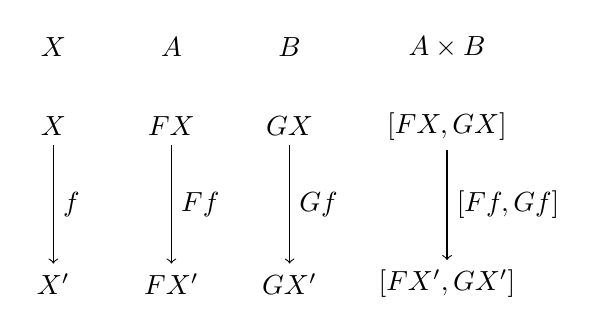
\begin{tikzpicture}[auto]
						\node (x) at (-1.5, 0) {$X$};
						\node (x') at (-1.5, -2) {$X'$};
						\node (a) at (0, 0) {$FX$};
						\node (a') at (0, -2) {$FX'$};
						\node (b) at (1.5, 0) {$GX$};
						\node (b') at (1.5, -2) {$GX'$};
						\node (ab) at (3.5, 0) {$[FX,GX]$};
						\node (ab') at (3.5, -2) {$[FX',GX']$};
						\draw[->] (x) to node{$f$}(x');
						\draw[->] (a) to node{$Ff$}(a');
						\draw[->] (b) to node{$Gf$}(b');
						\draw[->] (ab) to node{$[Ff,Gf]$}(ab');
						\node (cata) at (-1.5, 1) {$\cat{X}$};
						\node (cata) at (0, 1) {$\cat{A}$};
						\node (catb) at (1.5, 1) {$\cat{B}$};
						\node (catb) at (3.5, 1) {$\cat{A\times B}$};
					\end{tikzpicture}
				\end{center}
				\item[恒等射の保存]
				\begin{align*}
					\tuple{F,G}(id_X)&=\pcobj{F(id_X),G(id_X)}&\text{(射関数の定義)}\\
					&=\pcobj{id_{FX},id_{GX}}&\text{($F,G$の恒等射の保存)}\\
					&=id_{\pcobj{FX,GX}}&\text{(積圏の恒等射の定義)}
				\end{align*}
			よって恒等射を保つ
				\item[射の合成の保存]
				\begin{align*}
					\tuple{F,G}(f'\circ f)&=\pcobj{F(f'\circ f),G(f'\circ f)}&\text{(射関数の定義)}\\
					&=\pcobj{Ff'\circ Ff, Gf'\circ Gf}&\text{($F,G$の射の合成の保存)}\\
					&=\pcobj{Ff',Gf'}\circ\pcobj{Ff,Gf}&\text{(積圏の射の合成の定義)}\\
					&=\tuple{F,G}(f')\circ\tuple{F,G}(f)&\text{(射関数の定義)}
				\end{align*}
			よって射の合成を保つ。
			\end{mydescription}
		\end{quote}
	\end{define}
	\begin{prop}
		積圏$\cat{A\times B}$と射影関手$\Pi_\cat{A},\Pi_\cat{B}$の組$(\cat{A\times B},\Pi_\cat{A},\Pi_\cat{B})$は$\cat{Cat}$における積である。
	\end{prop}
	\begin{proof}
		積$(\cat{A\times B},\Pi_\cat{A},\Pi_\cat{B})$において、圏$\cat{X}$、関手$\functor{F}{X}{A}$、$\functor{G}{X}{B}$で構成される任意の組$(\cat{X},F,G)$に対して、$\Pi_\cat{A}\circ\tuple{F,G}=F,\ \Pi_\cat{B}\circ\tuple{F,G}=G$が成り立つような関手の対$\functor{\tuple{F,G}}{X}{A\times B}$が一意に存在することを示せばよい。
		\begin{center}
			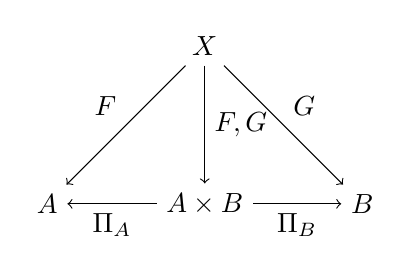
\begin{tikzpicture}[auto]
				\node (a) at (0, 0) {$\cat{A}$};
				\node (ab) at (2, 0) {$\cat{A\times B}$};
				\node (b) at (4, 0) {$\cat{B}$};
				\node (x) at (2, 2) {$\cat{X}$};
				\draw[->] (x) to node[swap]{$F$}(a);
				\draw[->] (x) to node{$G$}(b);
				\draw[->] (ab) to node{$\Pi_\cat{A}$}(a);
				\draw[->] (ab) to node[swap]{$\Pi_\cat{B}$}(b);
				\draw[->] (x) to node{$\tuple{F,G}$}(ab);
			\end{tikzpicture}
		\end{center}
		端的に述べるなら積圏、関手の対、射影関手の各々が持つ対象関数、射関数はそれぞれ積対象、射の対、射影射で構成されることから、積の普遍性を満たすことを示すのは難しくない。

		関手$F,G$の対象関数$F,G$、射影関手$\Pi_\cat{A},\Pi_\cat{B}$の対象関数$\pi_{\obj{A}},\pi_{\obj{B}}$、そして関手の対の対象関数$\tuple{F,G}$は、その定義により積の図式となる。
		すなわち対象関数$F,G$に対して対象関数$\tuple{F,G}$は一意に存在する。
		\begin{center}
			\begin{tikzpicture}[auto]
				\node (a) at (0, 0) {$\obj{A}$};
				\node (ab) at (4, 0) {$\obj{A}\times\obj{B}$};
				\node (abp) at (4, -1) {$\obj{A\times B}$};
				\node (b) at (8, 0) {$\obj{B}$};
				\node (x) at (4, 2) {$\obj{X}$};
				\draw[double distance=2pt] (ab) to (abp);
				\draw[->] (x) to node[swap]{$F$}(a);
				\draw[->] (x) to node{$G$}(b);
				\draw[->] (ab) to node{$\pi_{\obj{A}}$}(a);
				\draw[->] (ab) to node[swap]{$\pi_{\obj{B}}$}(b);
				\draw[->] (x) to node{$\tuple{F,G}$}(ab);
			\end{tikzpicture}
		\end{center}
		各射関数による積の図式は省略するが、同様に射関数$\tuple{F,G}$が一意に存在することが分かる。よって可換性を満たす対象関数と射関数も一意に存在することから、関手の対は積圏における射の対となり、$(\cat{A\times B},\Pi_\cat{A},\Pi_\cat{B})$は積の普遍性を満たす。
	\end{proof}
	\begin{define}[一点離散圏]
	一つの対象と一つの恒等射で構成される圏$\cat{1}$を\textbf{一点離散圏}とよぶ。
	\end{define}
	\begin{prop}[$\cat{Cat}$の終対象]
		$\cat{1}$は$\cat{Cat}$における終対象である。
	\end{prop}
	\begin{proof}
		任意の圏$\cat{C}$から一点離散圏$\cat{1}$への関手$!_{\cat{C}}$を考える。
		まず$\cat{1}$の対象$*$と射$id_*$は一つしか存在しない。そのため一点集合を$1$として
		\[\obj{1}=1,\ \arset{1}{*}{*}=1\]が成り立つ。

		よって対象関数$!_{\cat{C}}$は
		\begin{align*}
			&\mor{!_{\cat{C}}}{\obj{C}}{\obj{1}}\\
			=&\mor{!_{\cat{C}}}{\obj{C}}{1}
		\end{align*}
		となり一点集合への写像であることがわかる。よって任意の対象$A$に対して$!_{\cat{C}}(A)=*$が成り立ち、このような対象関数が一意に存在することが分かった。

		また任意の二対象$A,B$に対する射関数は
		\begin{align*}
			&\mor{{!_{\cat{C}}}_{A,B}}{\arset{C}{A}{B}}{\arset{1}{!_{\cat{C}}(A)}{!_{\cat{C}}(B)}}\\
			=&\mor{{!_{\cat{C}}}_{A,B}}{\arset{C}{A}{B}}{\arset{1}{*}{*}}\\
			=&\mor{{!_{\cat{C}}}_{A,B}}{\arset{C}{A}{B}}{1}\\
		\end{align*}と書ける。
		よって二対象$A,B$に対する各射関数も一意に存在することが分かった。

		関手$!_{\cat{C}}$の二つの写像が圏$\cat{C}$に対して一意に存在することわかる。
		よって任意の圏$\cat{C}$から一点離散圏$\cat{1}$への関手は一意に存在するから、一点離散圏$\cat{1}$は$\cat{Cat}$における終対象であることが示せた。
	\end{proof}
	\begin{prop}[対象と関手]
		任意の圏$\cat{C}$の元、つまり関手$\functor{A}{1}{C}$は圏$\cat{C}$の対象とみなせる。
	\end{prop}
	\begin{proof}
		関手$\functor{A}{1}{C}$は対象関数$\mor{F}{\obj{1}}{\obj{C}}$、射関数$\mor{F}{\arset{1}{*}{*}}{\arset{C}{F(*)}{F(*)}}$で構成される。このとき、$\obj{1}$は一点集合であるから、対象関数$F$は$\obj{C}$の元である。

		また射関数も同様に$\arset{C}{F(*)}{F(*)}$の元であるが、恒等射の保存より写される射は恒等射ただ一つであり、射関数は対象関数に対して一通りにしか定義できないから考慮しなくてもよい。

		よって関手$\functor{A}{1}{C}$は圏$\cat{C}$の対象とみなせる。
	\end{proof}
  集合の圏では$A\cong\arset{Set}{1}{A}$が成り立ったから、$\cat{Cat}$でも$\cat{A}\cong\arset{Cat}{\cat{1}}{\cat{A}}$のような主張が成り立つと考えるかもしれないが、$\arset{Cat}{\cat{1}}{\cat{A}}$はただの射集合、関手の集合であり、$\cat{Cat}$の対象にはならないから同型射となる関手を取ることができない。その上、この関手の集合は対象の集合であり圏の射の情報は全く含まれない。そのためこのような同型を考えるには$\cat{Cat}$における射集合的な圏を考える必要がある。この問題は後に関手圏と呼ばれる圏を定義することで解決する。

	関手としての対象の話に戻ると、積圏$\cat{A\times B}$の対象を$\pcobj{A,B}$と表したが、実際に対象$\functor{A}{1}{A}$と対象$\functor{B}{1}{B}$の関手の対$\functor{\tuple{A,B}}{1}{A\times B}$は$\cat{A\times B}$の対象になる。
